\section{Platform Analysis}



Figures \ref{fig:platform_heatmap_group1}, \ref{fig:platform_heatmap_group2}, and \ref{fig:platform_heatmap_group3} show performance comparison between LeetCode and AtCoder platforms across different programming languages. Models demonstrate varying capabilities depending on the platform, with some excelling on LeetCode's interview-style problems while others perform better on AtCoder's competitive programming tasks. 

\begin{figure}[hbt]
    \centering
    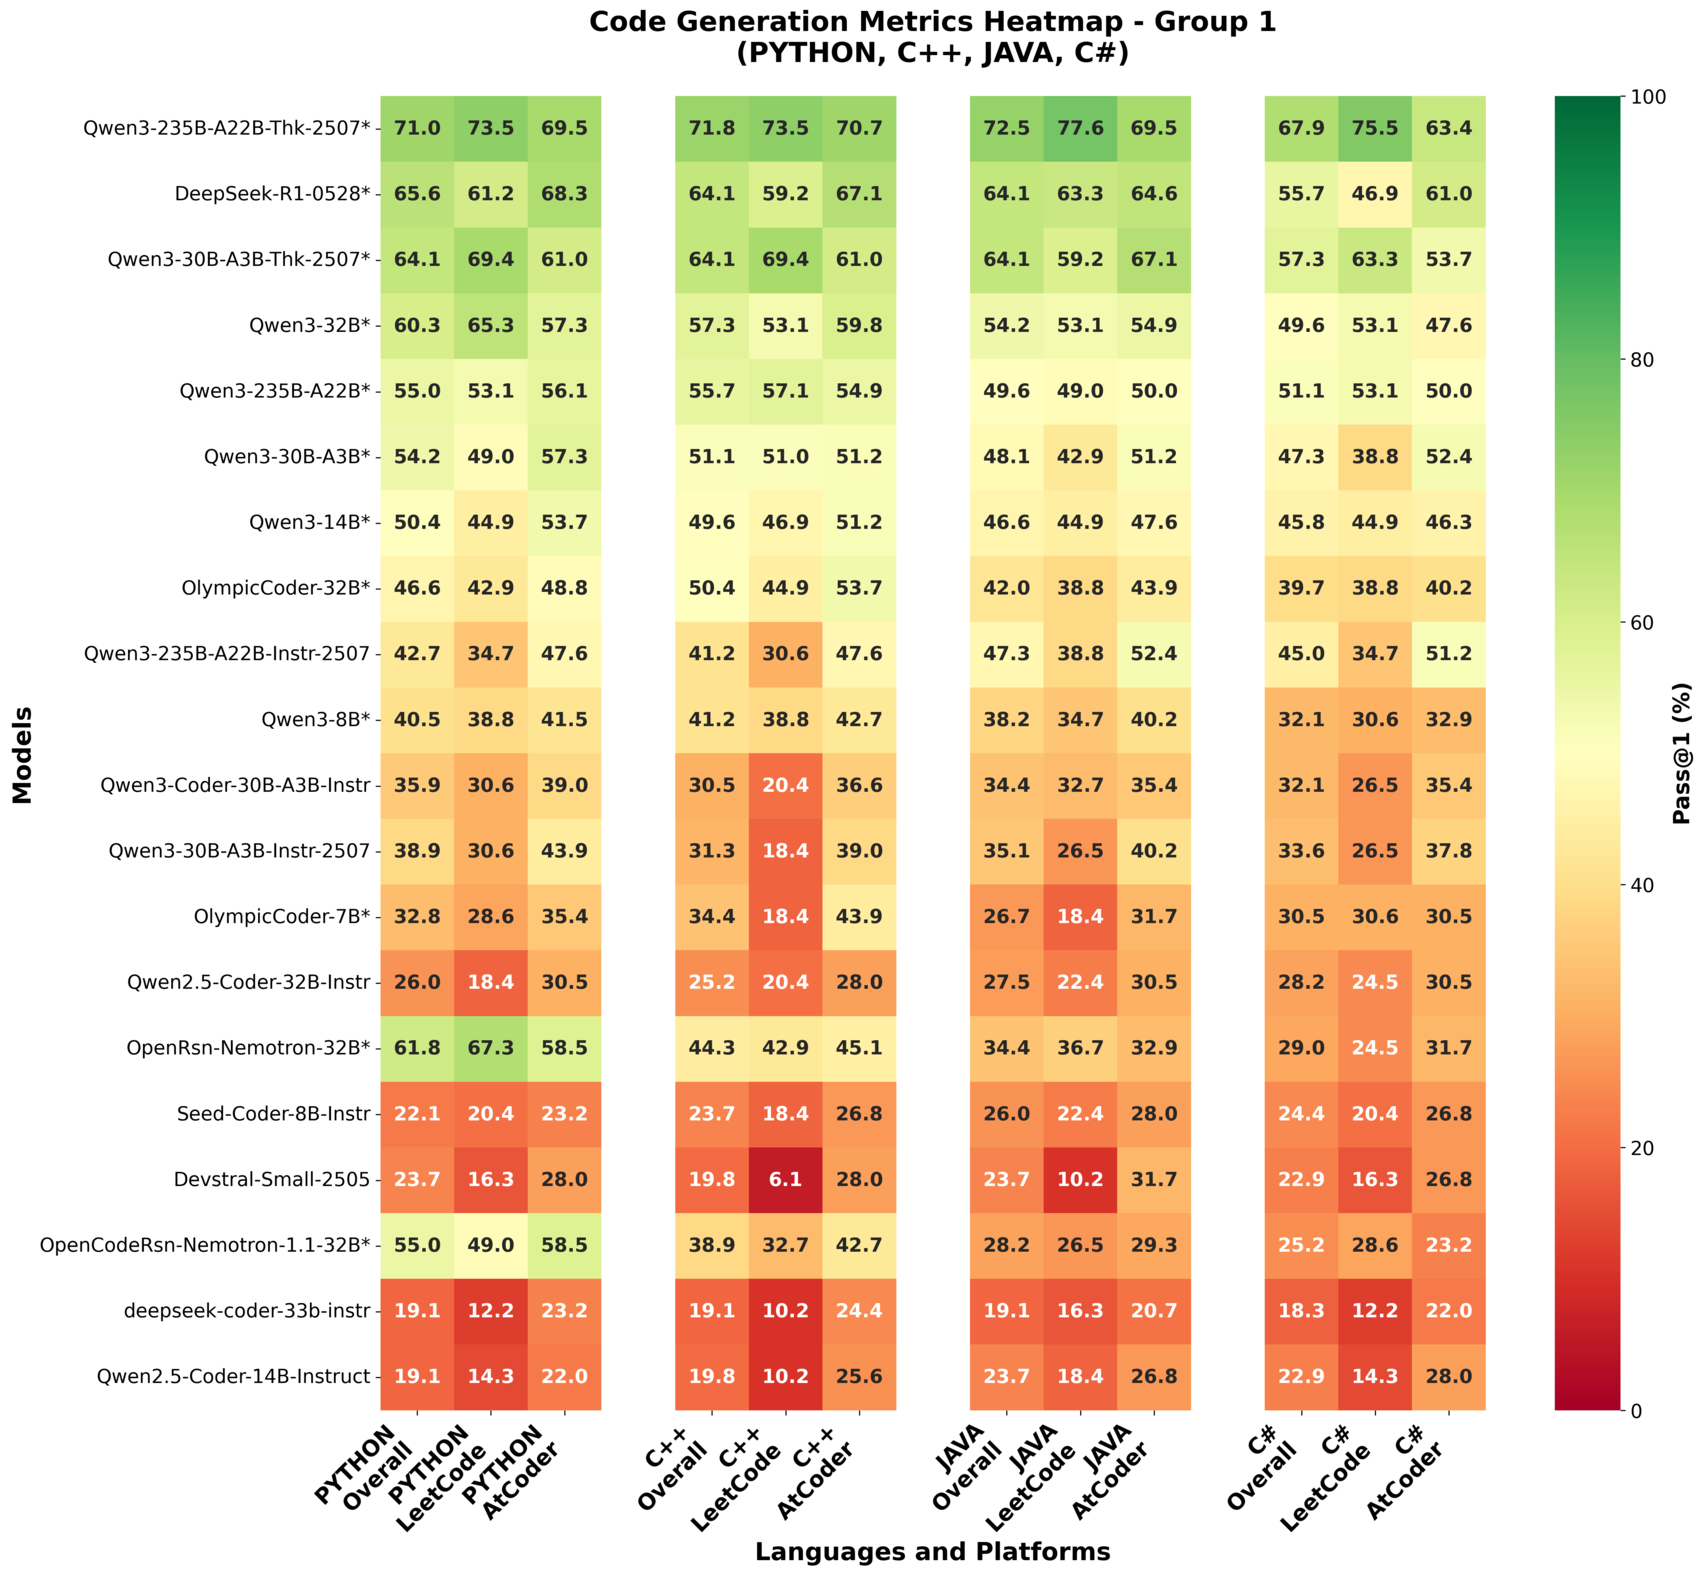
\includegraphics[width=1\linewidth]{figs//heatmap_by_platform/metrics_heatmap_group_1.png}
    \caption{Code generation performance heatmap by platform for Python, C++, Java, and C\#. Shows overall performance and platform-specific results (LeetCode vs AtCoder) across different models. Values represent Pass@1 scores (\%).}
    \label{fig:platform_heatmap_group1}
\end{figure}

\begin{figure}
    \centering
    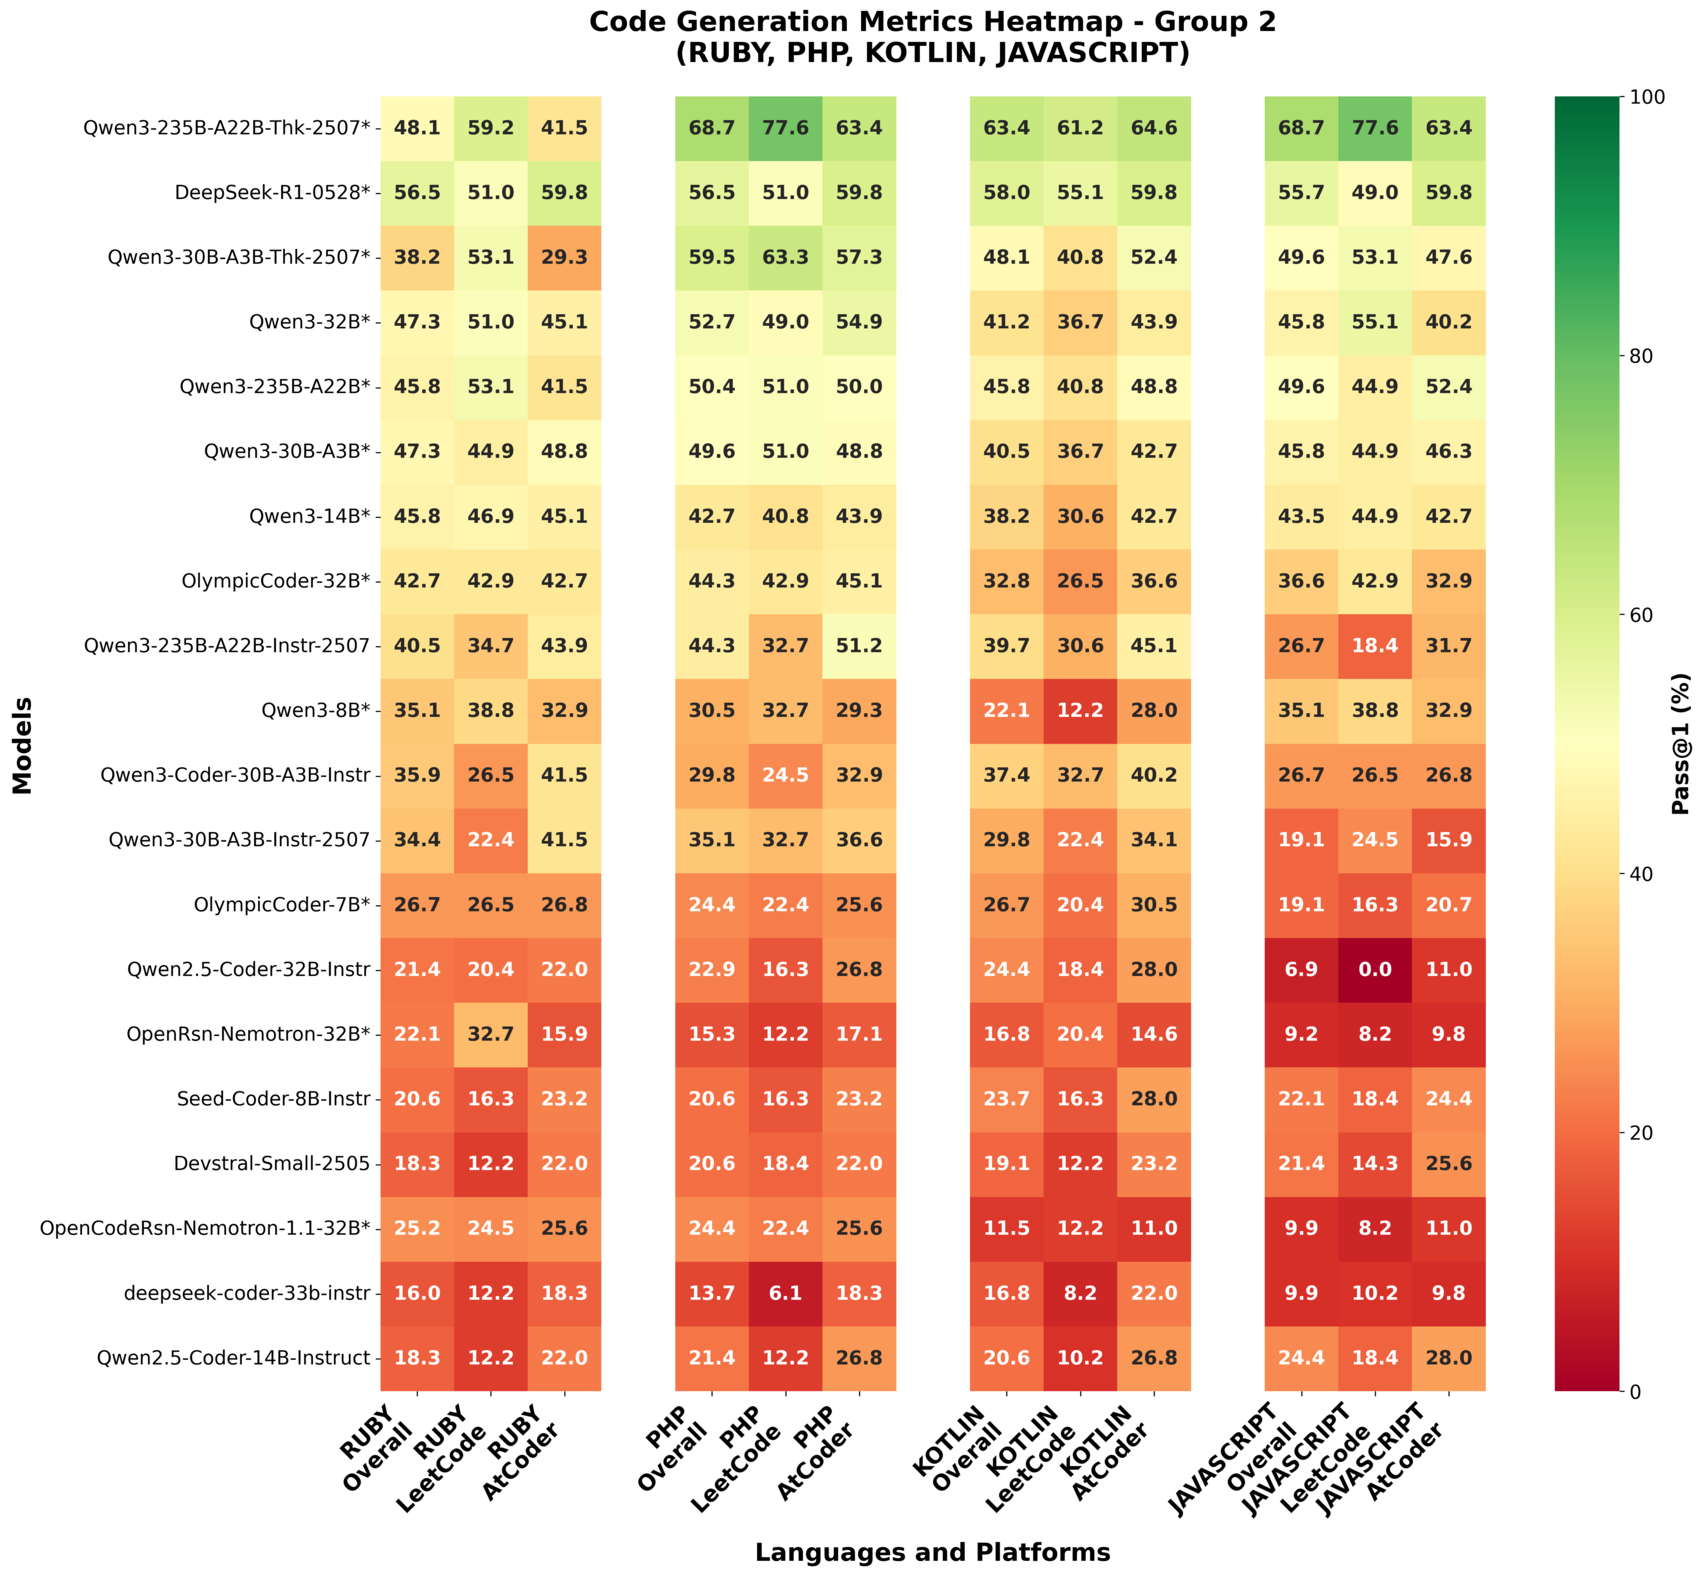
\includegraphics[width=1\linewidth]{figs//heatmap_by_platform/metrics_heatmap_group_2.png}
    \caption{Code generation performance heatmap by platform for Ruby, PHP, Kotlin, and JavaScript. Shows overall performance and platform-specific results (LeetCode vs AtCoder) across different models. Values represent Pass@1 scores (\%).}
    \label{fig:platform_heatmap_group2}
\end{figure}

\begin{figure}
    \centering
    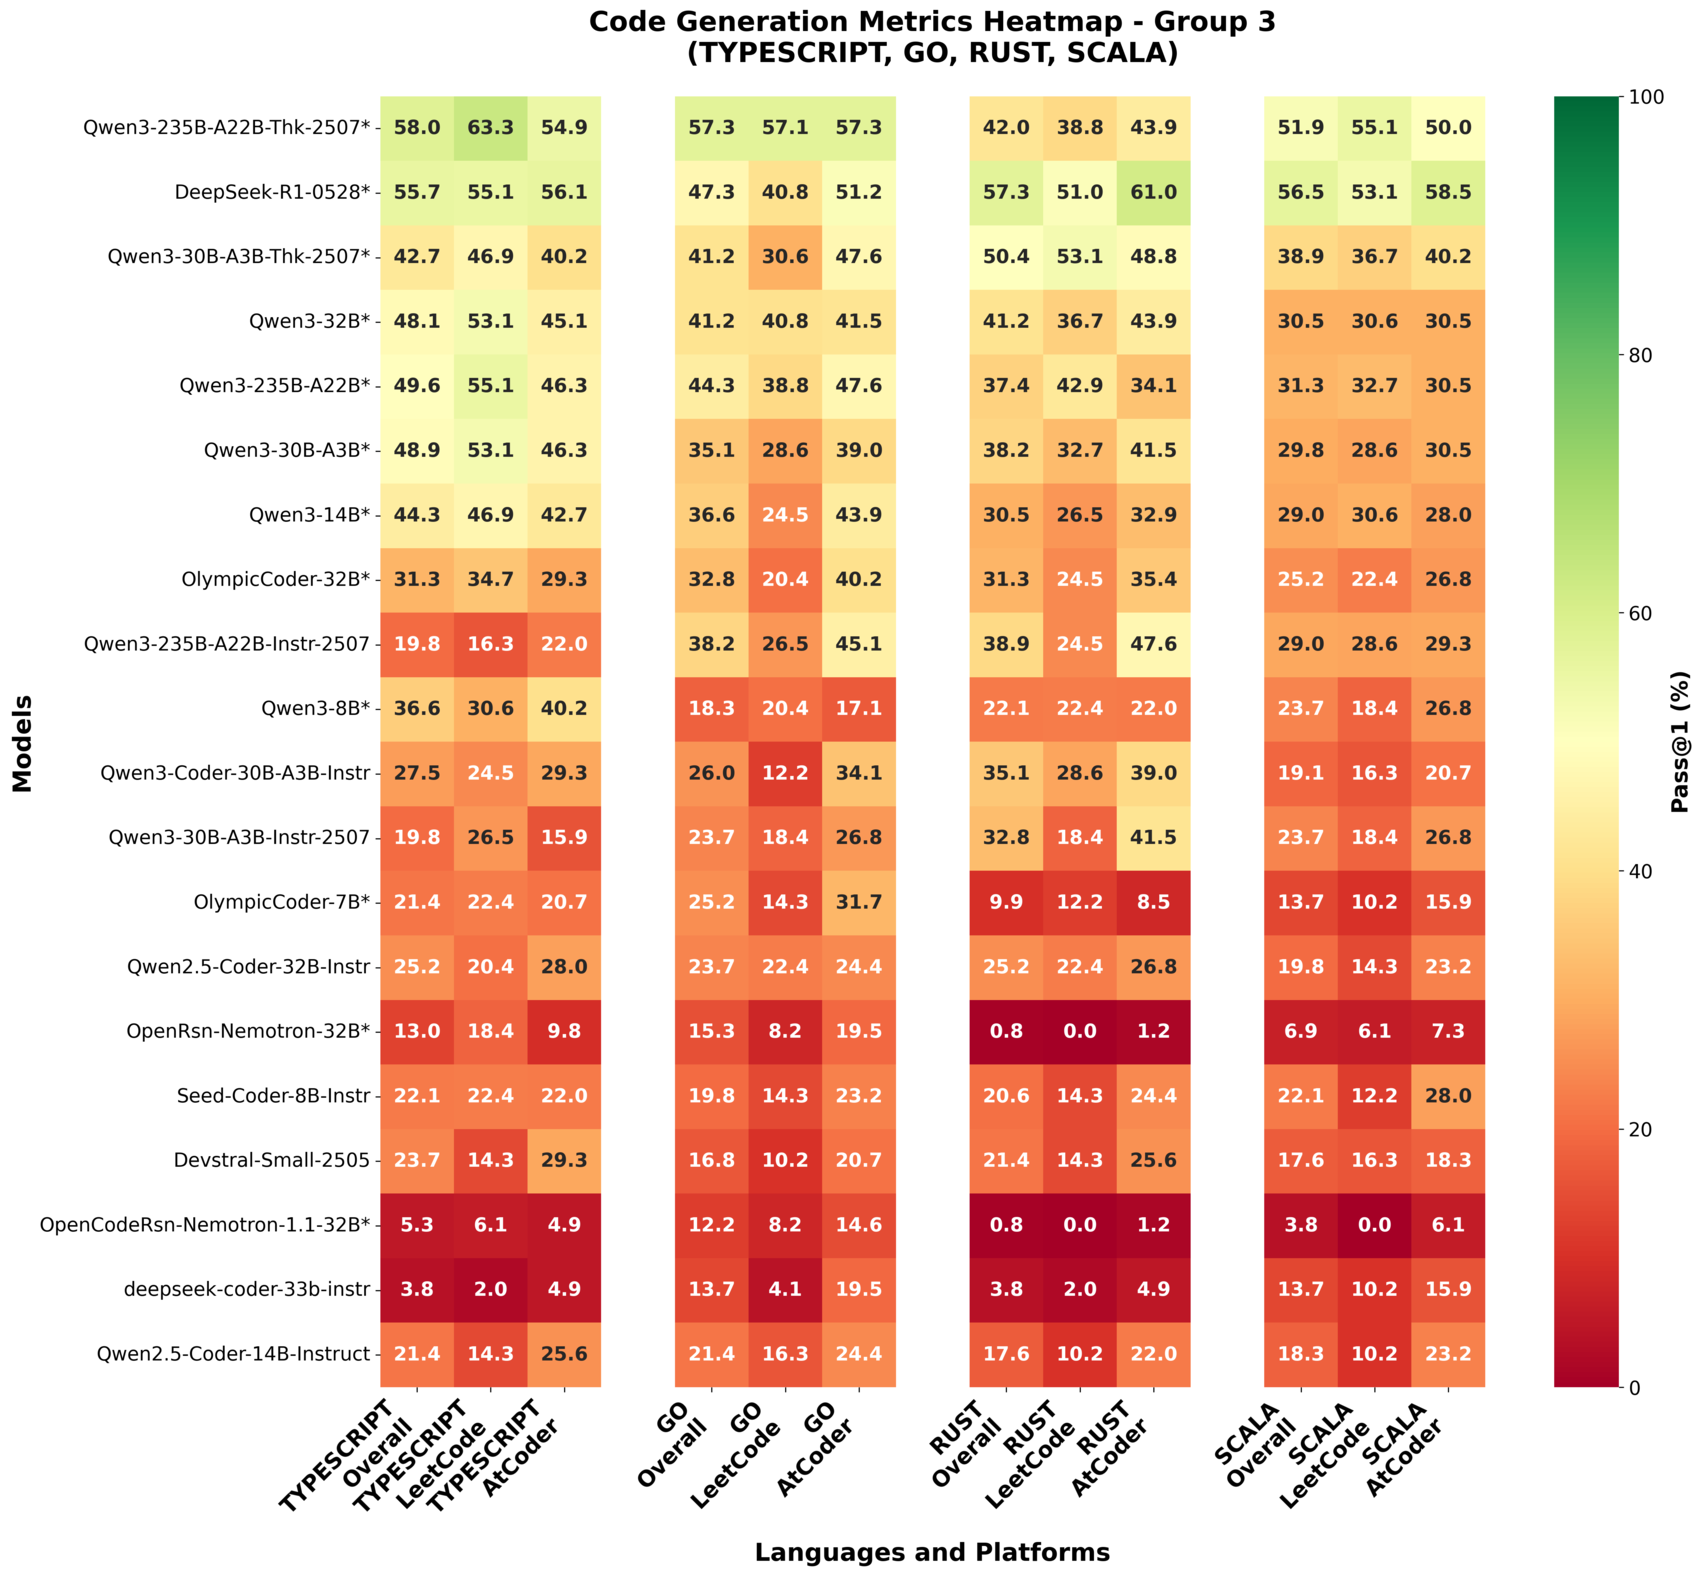
\includegraphics[width=1\linewidth]{figs//heatmap_by_platform/metrics_heatmap_group_3.png}
    \caption{Code generation performance heatmap by platform for TypeScript, Go, Rust, and Scala. Shows overall performance and platform-specific results (LeetCode vs AtCoder) across different models. Values represent Pass@1 scores (\%).}
    \label{fig:platform_heatmap_group3}
\end{figure}
\clearpage

% by task type 

% \begin{figure}
%     \centering
%     \includegraphics[width=1\linewidth]{figs/by_task_type/task_type_heatmap_group_1.png}
%     \caption{Enter Caption}
%     \label{fig:placeholder}
% \end{figure}

% \begin{figure}
%     \centering
%     \includegraphics[width=1\linewidth]{figs/by_task_type/task_type_heatmap_group_2.png}
%     \caption{Enter Caption}
%     \label{fig:placeholder}
% \end{figure}

% \begin{figure}
%     \centering
%     \includegraphics[width=1\linewidth]{figs//by_task_type/task_type_heatmap_group_3.png}
%     \caption{Enter Caption}
%     \label{fig:placeholder}
% \end{figure}



\section{Difficulty Analysis}



Figures \ref{fig:difficulty_heatmap_group1}, \ref{fig:difficulty_heatmap_group2}, and \ref{fig:difficulty_heatmap_group3} present performance breakdown by difficulty levels (Easy, Medium, Hard) across programming languages. The results reveal significant performance degradation as problem complexity increases, with Hard problems showing the largest performance gaps between models.


\begin{figure}[hbt]
    \centering
    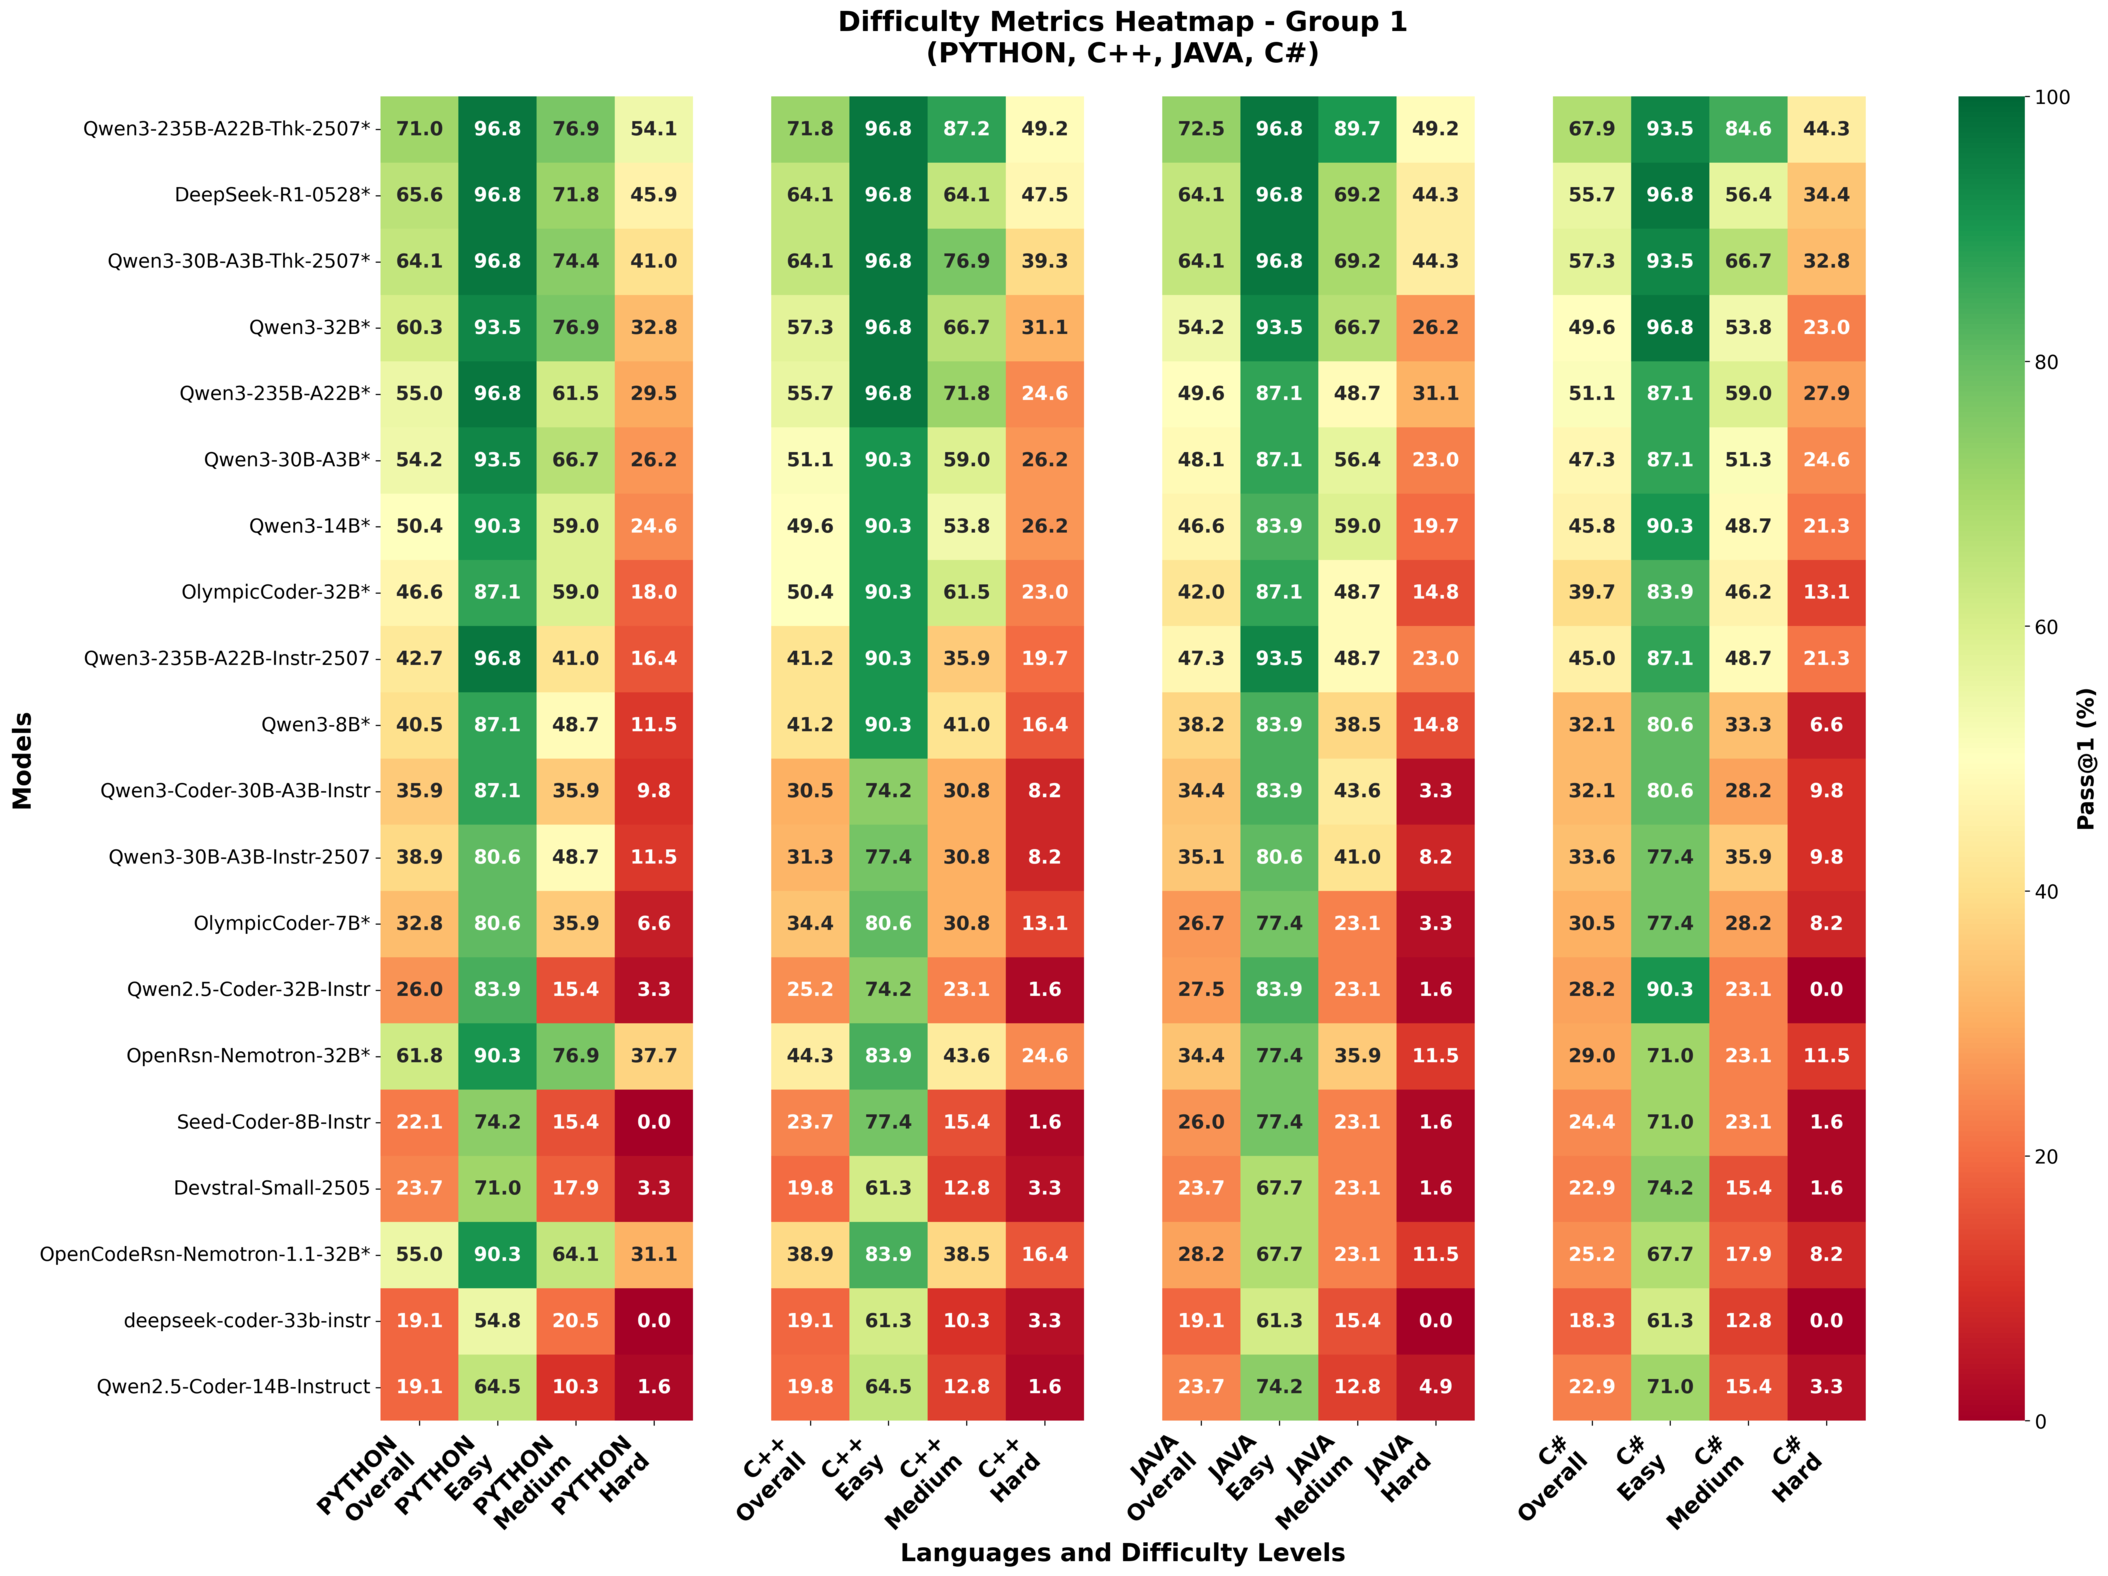
\includegraphics[width=1\linewidth]{figs/heatmap_by_difficulty/difficulty_heatmap_group_1.png}
    \caption{Code generation performance heatmap by difficulty level for Python, C++, Java, and C\#. Shows overall performance and difficulty-specific results (Easy, Medium, Hard) across different models. Values represent Pass@1 scores (\%).}
    \label{fig:difficulty_heatmap_group1}
\end{figure}

\begin{figure}
    \centering
    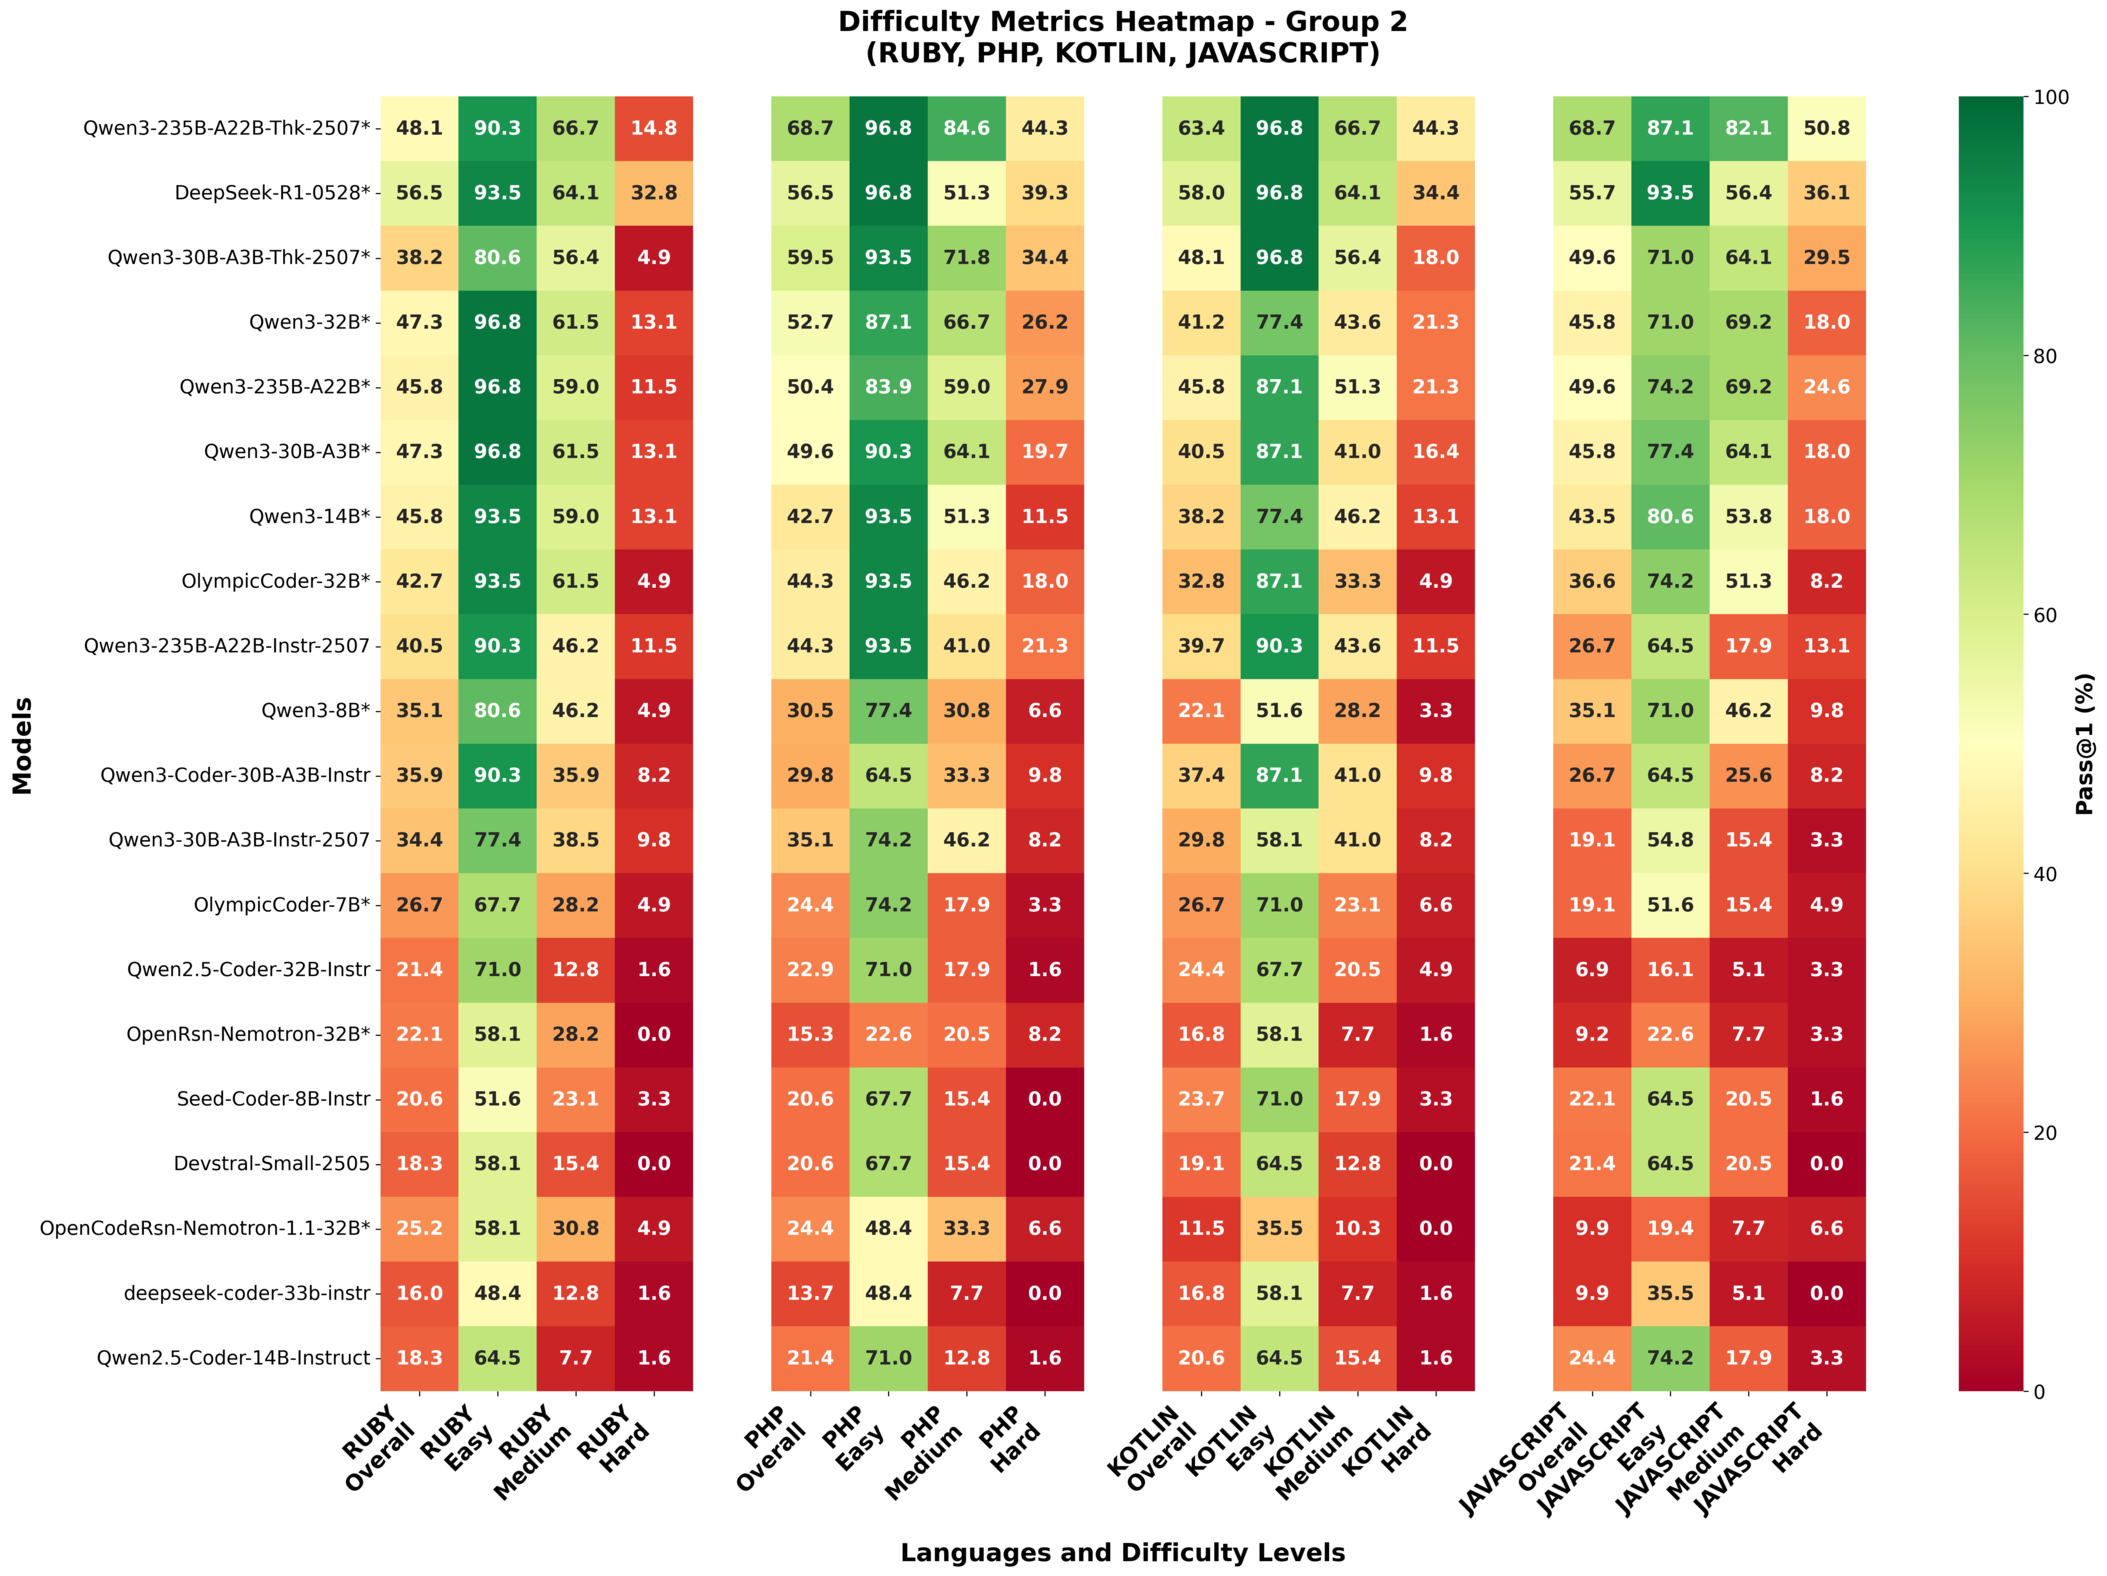
\includegraphics[width=1\linewidth]{figs/heatmap_by_difficulty/difficulty_heatmap_group_2.png}
    \caption{Code generation performance heatmap by difficulty level for Ruby, PHP, Kotlin, and JavaScript. Shows overall performance and difficulty-specific results (Easy, Medium, Hard) across different models. Values represent Pass@1 scores (\%).}
    \label{fig:difficulty_heatmap_group2}
\end{figure}

\begin{figure}
    \centering
    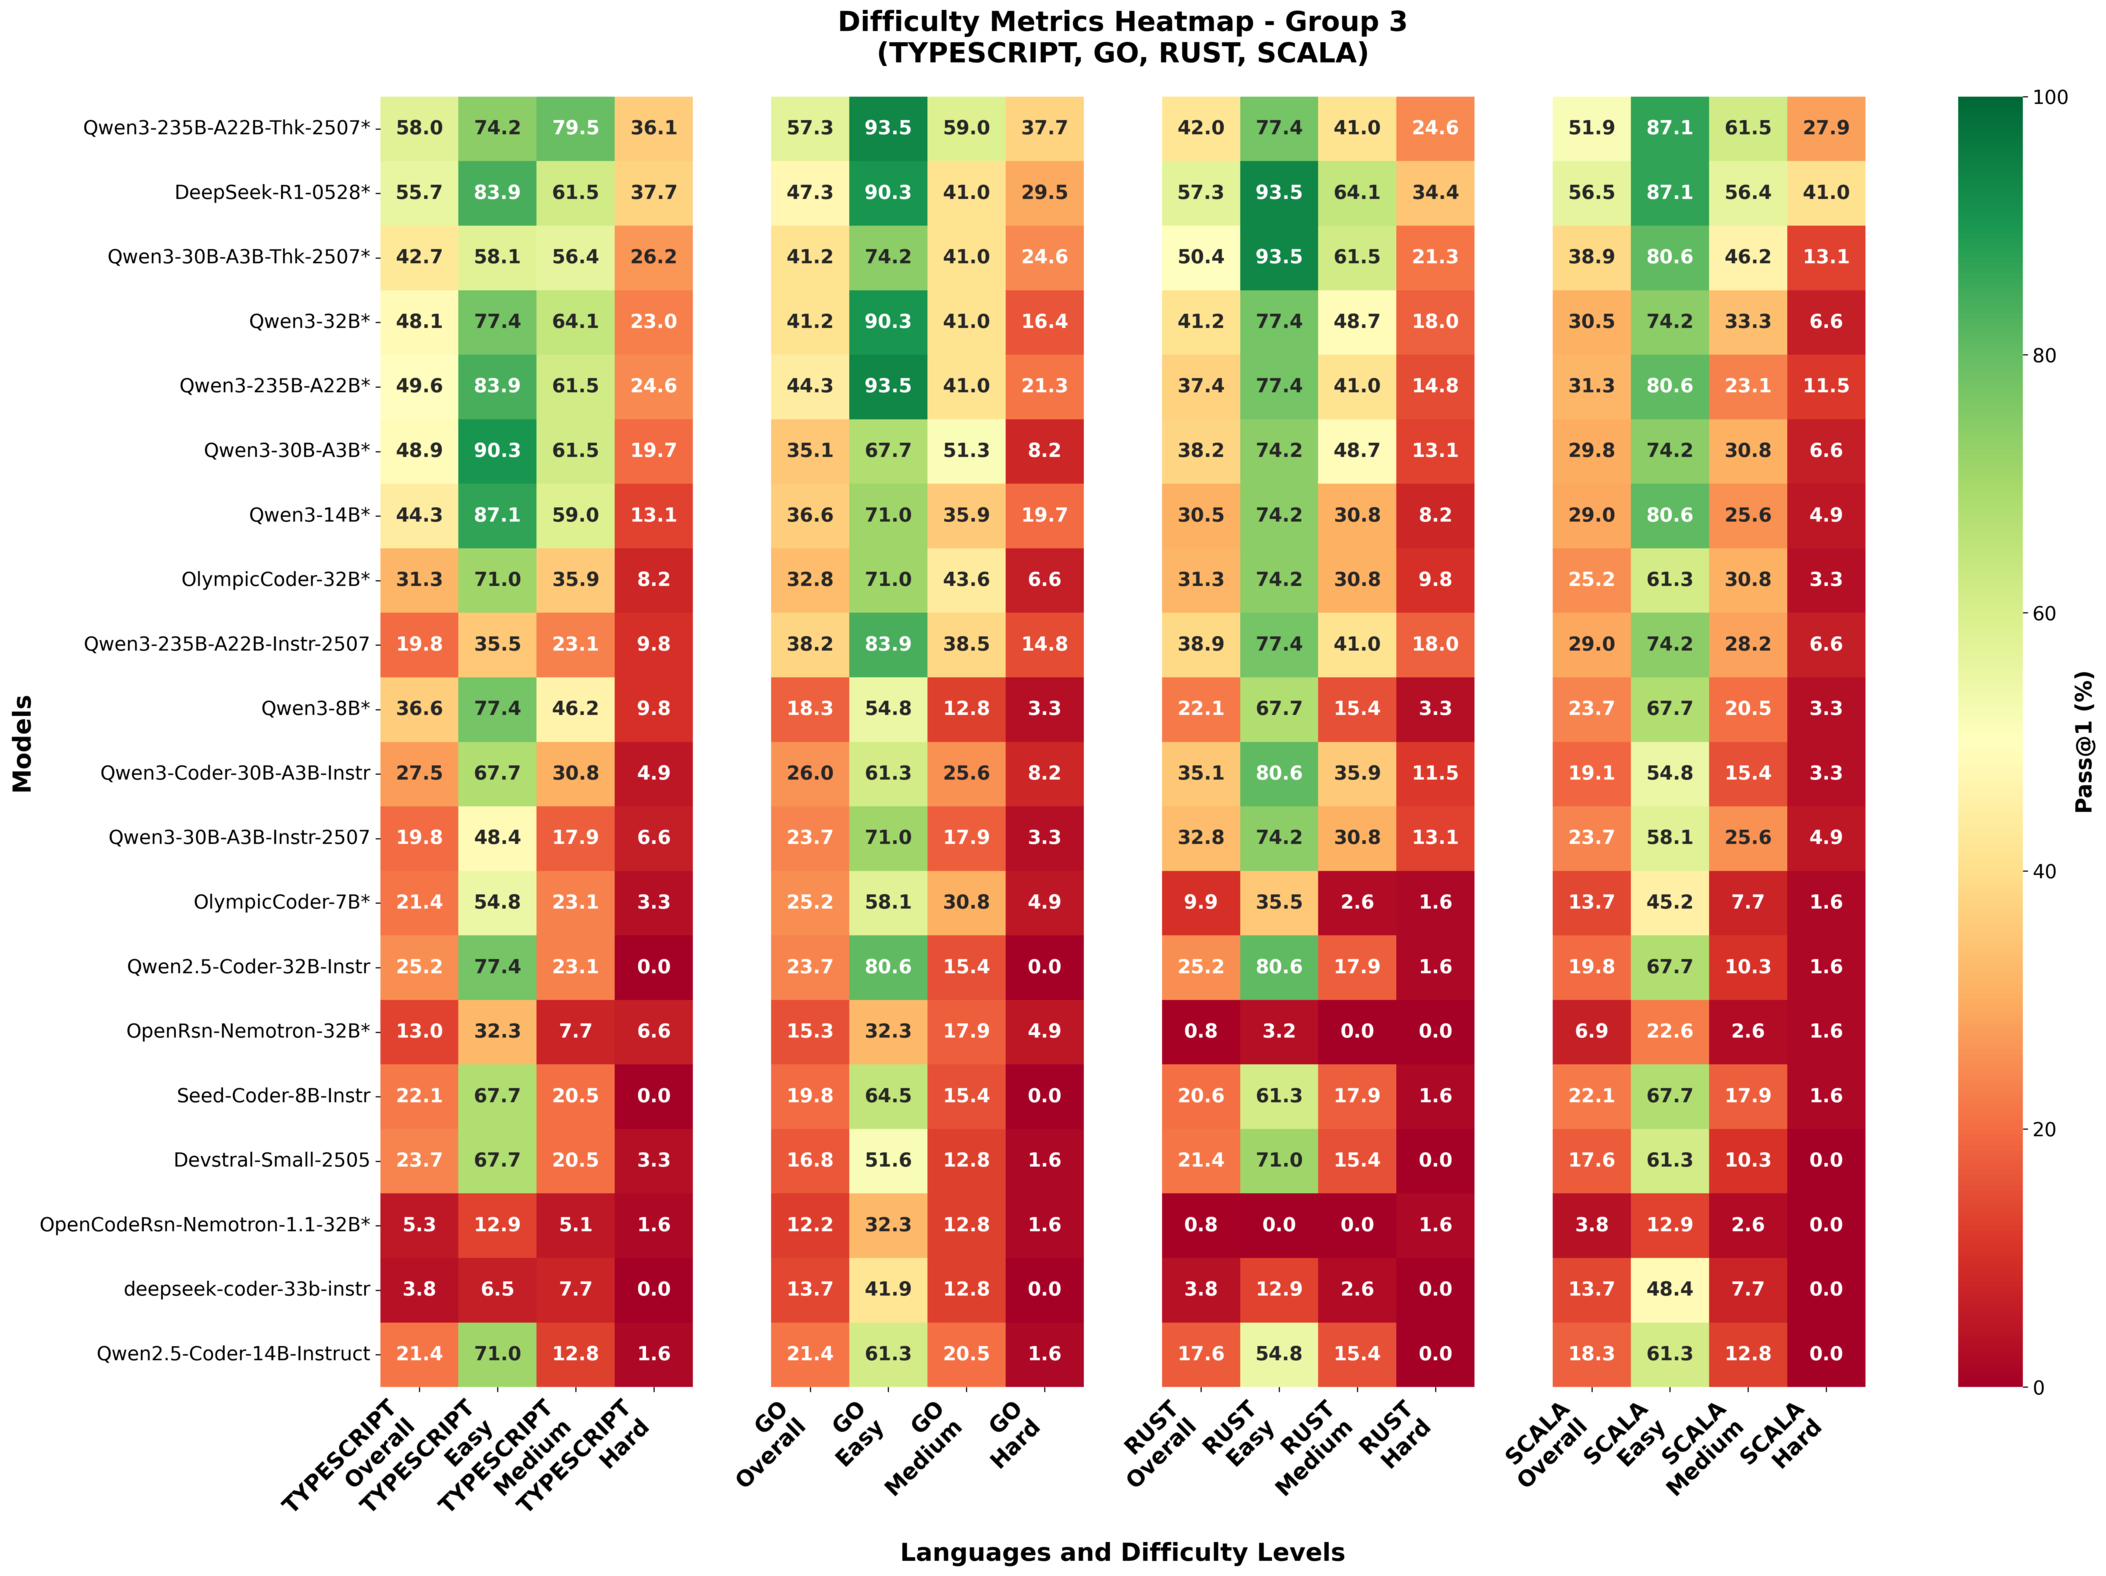
\includegraphics[width=1\linewidth]{figs/heatmap_by_difficulty/difficulty_heatmap_group_3.png}
    \caption{Code generation performance heatmap by difficulty level for TypeScript, Go, Rust, and Scala. Shows overall performance and difficulty-specific results (Easy, Medium, Hard) across different models. Values represent Pass@1 scores (\%).}
    \label{fig:difficulty_heatmap_group3}
\end{figure}


\clearpage
